\documentclass[xcolor=dvipsnames]{beamer}

\usepackage{mpctools}

\setbeamertemplate{navigation symbols}{}

\begin{document}
%
\begin{frame}[allowframebreaks]{Windows/Linux Installation}
    Install a scientific Python distribution
    \begin{itemize}
        \item Any ``Scientific Python'' should do, but it must include NumPy, SciPy, and matplotlib.
        \item For Windows, e.g., Python(x,y): \smallurl{https://code.google.com/p/pythonxy/}
        \item For Ubuntu/Debian, e.g., Spyder (an IDE): \lstinline[style=shell]@sudo apt-get install spyder@
    \end{itemize}
    
    \medskip
    
    Download \casadi 2.3.0
    \begin{itemize}
        \item Windows/Linux zip file available at \smallurl{http://sourceforge.net/projects/casadi/files/CasADi/}
        \item Unzip to a convenient location (e.g., \smallurl{C:/Python2.7/casadi} for Windows or \smallurl{/opt/casadi} for Casadi)
    \end{itemize}
    
    \framebreak
    
    Download our \texttt{mpctools} Python package
    \begin{itemize}
        \item Download Mercurial repo (zip link on left): \smallurl{https://hg.cae.wisc.edu/hg/mpc-tools-casadi}
        \item Unzip to a convenient location.
        \item Move the \texttt{mpctools} sub-folder to where you unzipped \texttt{casadi}; the remaining files (examples and documentation) can be left where they are.
    \end{itemize}
    
    \medskip
    
    Add CasADi and \texttt{mpctools} to your Python path
    \begin{itemize}
        \item Open a Python interpreter (run \lstinline[style=shell]!python! from a terminal/command prompt)
        \item Run the commands \lstinline[style=python]!import site; print site.getsitepackages()! to see where your site packages are stored
        \item In one of the site package folders, make a text file called \texttt{casadi.pth}, and type the path to your CasADi installation directory
    \end{itemize}
\end{frame}

\begin{frame}{Mac Installation (Difficult)}
       Install Python, NumPy, SciPy, matplotlib
       \begin{itemize}
           \item E.g., via Homebrew: \lstinline[style=shell]!brew install python!
           \item Packages via \texttt{pip}: \lstinline[style=shell]!pip install ipython matplotlib numpy scipy
           !
        \end{itemize}
        
        \medskip
        
        Build and Install CasADi 2.3.0
        \begin{itemize}
            \item You'll have to build from sources.
            \item See \smallurl{https://github.com/casadi/casadi/wiki/InstallationMac} for details.
            \item We can only provide minimal support for this option.
        \end{itemize}
        
        \medskip
        
        Our Python package
        \begin{itemize}
            \item Download Mercurial repo: \smallurl{https://hg.cae.wisc.edu/hg/mpc-tools-casadi}
            \item Unzip and move the \texttt{mpctools} folder to somewhere on your Python Path
        \end{itemize}
\end{frame}

\begin{frame}{Making Sure Everything Works}
    First, open a Python interpreter\footnote{Open a command prompt/terminal in the \smallurl{mpc-tools-casadi} folder and enter \lstinline[style=shell]!python!. You may also be able to right-click and choose ``Open a Python console''.} and run \lstinline[style=python]!import casadi, mpctools!.
    \begin{itemize}
        \item If this doesn't work, make sure your CasADi folder shows up in \lstinline[style=python]!import sys; print sys.path!.
        \item If you have multiple Python distributions on your machine, don't (or at least make sure you're using the one you think you are).
        \item Make sure you are using Python 2.7 (not 3.x).
    \end{itemize}
        
    Then, try to run the examples in \smallurl{mpc-tools-casadi}.
    \begin{itemize}
        \item In the Python interpreter, use \lstinline[style=python]!execfile("filename.py")!.
        \item \smallurl{runall.py} will run everything and tell you if there are errors, but you won't see any plots.
    \end{itemize}
\end{frame}


\begin{frame}{Software Relationships}
    \centering
    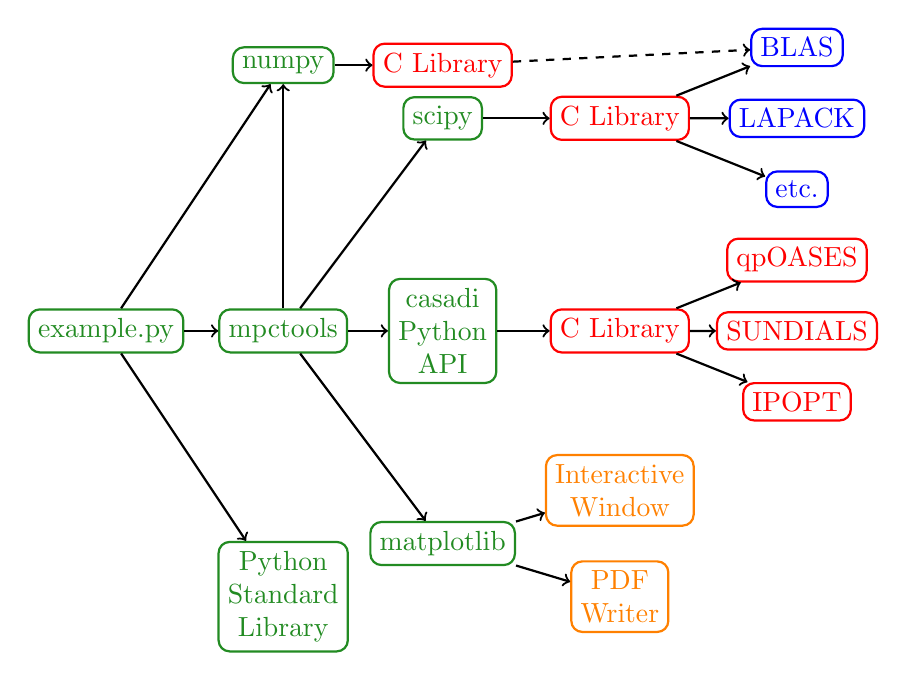
\begin{tikzpicture}
        [
            grow=right,
            code/.style={rectangle,rounded corners,align=center,thick},
            python/.style={code,draw=ForestGreen,text=ForestGreen},
            clib/.style={code,draw=Red,text=Red},
            fortran/.style={code,draw=Blue,text=Blue},
            backend/.style={code,draw=orange,text=orange},
            level 1/.style={level distance=2.5cm,sibling distance=3.75cm},
            level 2/.style={level distance=2.25cm,sibling distance=3cm},
            level 3/.style={level distance=2.5cm,sibling distance=1.5cm},
            level 4/.style={level distance=2.5cm,sibling distance=1cm},
            level 5/.style={level distance=2.5cm,sibling distance=1cm},
            arw/.style={->,thick},
            scale=.9,
        ]
        \draw (0,0) node[python] {example.py}
        child
        {
            node[python] {Python\\Standard\\Library}
            edge from parent [arw]
        }
        child
        {
            node[python] (mpc) {mpctools}
            child
            {
                node[python] (matplotlib) {matplotlib}
                child
                {
                    node [backend] {PDF\\Writer}
                    edge from parent [arw]
                }
                child
                {
                    node [backend] {Interactive\\Window}
                    edge from parent [arw]
                }
                edge from parent [arw]
            }
            child
            {
                node[python] (casadipy) {casadi\\Python\\API}
                child
                {
                    node[clib] {C Library}
                    child
                    {
                        node[clib] {IPOPT}
                        edge from parent [arw]
                    }
                    child
                    {
                        node[clib] {SUNDIALS}
                        edge from parent [arw]
                    }
                    child
                    {
                        node[clib] {qpOASES}
                        edge from parent [arw]
                    }
                    edge from parent [arw]
                }
                edge from parent [arw]
            }
            child
            {
                node[python] (scipy) {scipy}
                child
                {
                    node[clib] {C Library}
                    child
                    {
                        node[fortran] {etc.}
                        edge from parent [arw]
                    }
                    child
                    {
                        node[fortran] {LAPACK}
                        edge from parent [arw]
                    }
                    child
                    {
                        node[fortran] (blas) {BLAS}
                        edge from parent [arw]
                    }
                    edge from parent [arw]
                }
                edge from parent [arw]
            }
            edge from parent [arw]
        }
        child
        {
            node[python] (numpy) {numpy}
            child
            {
                node[clib] (numpylib) {C Library}
                edge from parent [arw]
            }
            edge from parent [arw]
        };
        \draw[arw] (mpc) -- (numpy);
        \draw[arw,dashed] (numpylib) -- (blas);
    \end{tikzpicture}
\end{frame}
%
%
\end{document}